\subsection{Activation} \label{subs:acti}
The activation function is the non-linear output of the neuron. Its purpose is to decide whether the neuron fires or not. To apply the back-propagation algorithm (see Section \ref{sec:train}), which makes the network learn, we need to have the activation function to be differentiable \cite{lecun_backpropagation_1989}. To optimize the network, we must compute the gradient of the activation function. As the step function described in equation \eqref{eq:step} has a gradient of zero, the perceptron can not learn if we use this activation function. Various activation functions have then been proposed with different properties, as illustrated in Figure \ref{fig:acti}. According to \textcite{khan_survey_2020}, the choice of an appropriate activation function can accelerate the learning phase and some activations have less computational complexity \cite{krizhevsky_imagenet_2012}.
%
\begin{figure}
    \centering
    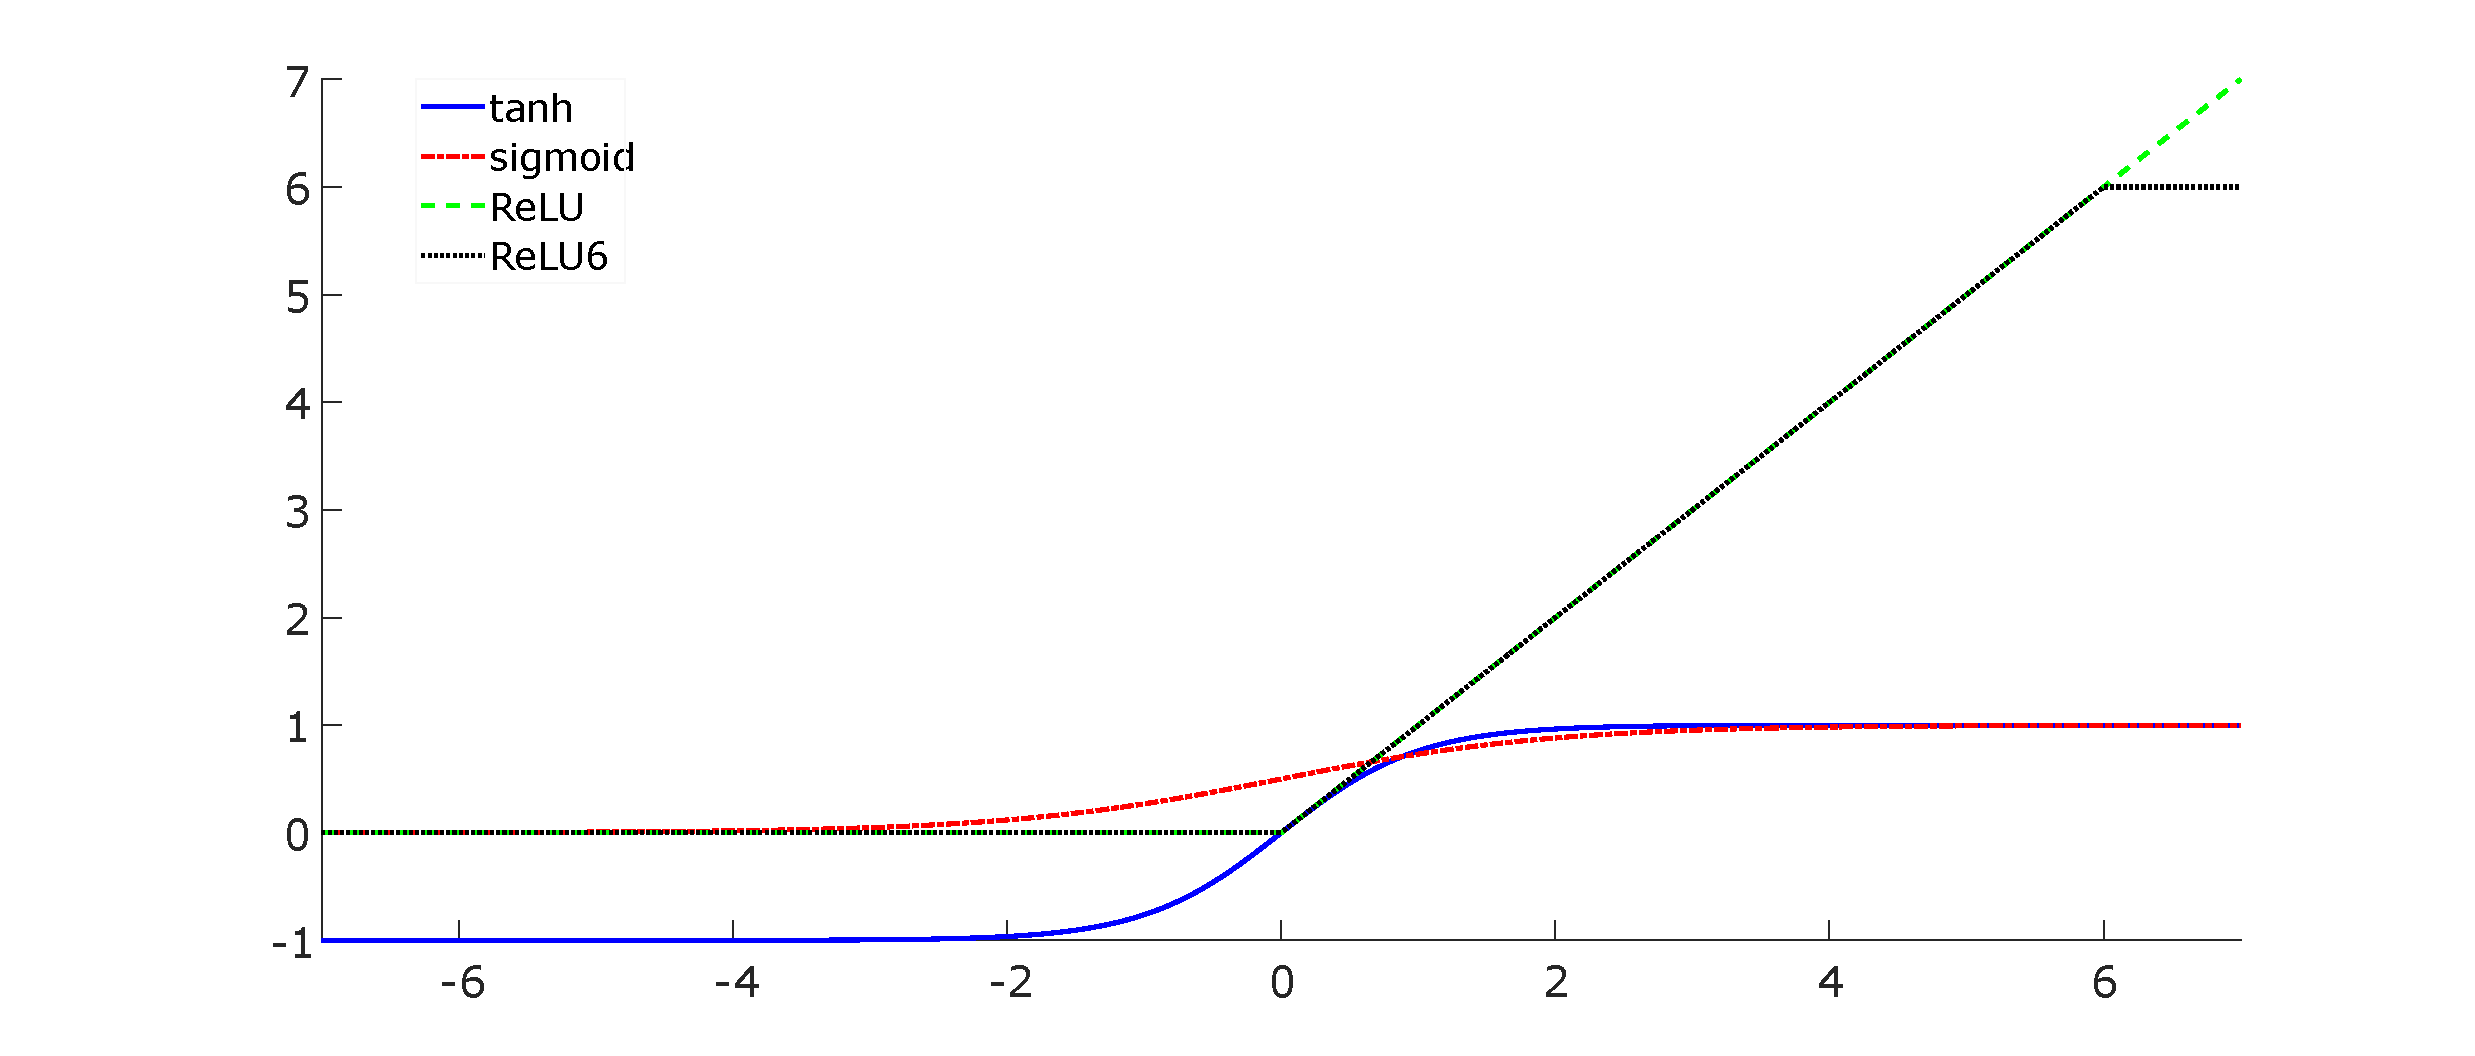
\includegraphics[width=\textwidth]{actifun.pdf}
    \caption{Activation functions}
    \label{fig:acti}
\end{figure}
%
\subsubsection{Sigmoid and Hyperbolic Tangent (Tanh)}
$Sigmoid$ and $Thanh$ are both smooth functions that can be described by equations \eqref{eq:sigmoid} and \eqref{eq:tanh}.
%
\begin{equation}
    h(x) = \frac{1}{1 + e^{-x}}
    \label{eq:sigmoid}
\end{equation}
%
\begin{equation}
    h(x) = \frac{e^{x} - e^{-x}}{e^{x} + e^{-x}}
    \label{eq:tanh}
\end{equation}
%
The two activation functions can be seen in Figure \ref{fig:acti}. They both \textquote{squeeze} the domain $\mathbb{R}$ into a smaller range, $[0, 1]$ for $Sigmoid$, and $[-1, 1]$ for the $Tanh$. However, they also saturate at the asymptotes, which means that often their gradient is close to 0. As the back-propagation algorithm requires gradient multiplication, gradient far away from the output vanishes (close to 0) and deep models do not learn: it is the \textbf{vanishing gradient problem} \cite{goodfellow_deep_2016}.
%
\subsubsection{ReLU}
To solve the problem of saturation, the Rectified Linear Unit (ReLU) has been introduced by \textcite{krizhevsky_imagenet_2012}. Equation \eqref{eq:relu} describes its behavior.
\begin{equation}
    h(x) = max(0, x)
    \label{eq:relu}
\end{equation}
%
This activation function allows faster learning, efficient gradient propagation (no vanishing or exploding gradient), and a faster computation than $Thanh$ or $Sigmoid$. However, it suffers from the \textbf{dying neuron problem} which decreases the model capacity. Some neurons become inactive (output only 0) for essentially all inputs and they \textquote{die}. A neuron that only outputs zero can be discarded. A solution would be to modify the ReLU like leaky ReLU \cite{maas_rectier_2014}, etc.

Other works try to modify the ReLU for implementation on embedded platforms. For example, \cite{howard_mobilenets_2017} uses ReLU6 (equation \eqref{eq:relu6}), which we can see in Figure \ref{fig:acti}. It is designed for fixed-point operations and quantization approaches, instead of floating-point operations which are less efficient in terms of hardware utilization and power consumption (especially on \acrshort{fpga}) \cite{david_hardware_2007}. More information about quantification can be found in Section \ref{subsec:mdopti}. Therefore, if the output $\in [ 0, 6 ]$, the number of bits for the integer part can be limited to 3 bits. We can thus increase the accuracy of the model by assigning the other bits to the decimal part.
%
\begin{equation}
    h(x) = max(0, x, 6)
    \label{eq:relu6}
\end{equation}
